\graphicspath{{images/}}

\section{\thesection~Methods}
\label{sec:methods}

\subsection{\thesubsection~Subsection}

\begin{Figure}
  \centering
  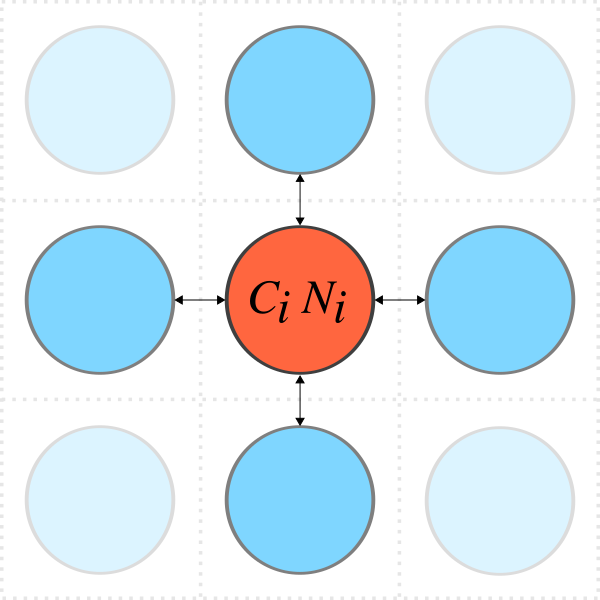
\includegraphics[width=\linewidth]{comp_model/comp_model_schematic}
  \captionof{figure}{Schematic of the modelling approach. Each circle
    represents a culture, indexed \(i\), on solid agar and arrows represent diffusion
    of nutrients. \(C_{i}\) - amount of cells;
    \(N_{i}\) - amount of nutrients; darker blue circles-
    neighbourhood \(\delta_{i}\).}
  \label{fig:comp_model_schematic}
\end{Figure}


\begin{Figure}
  \centering
  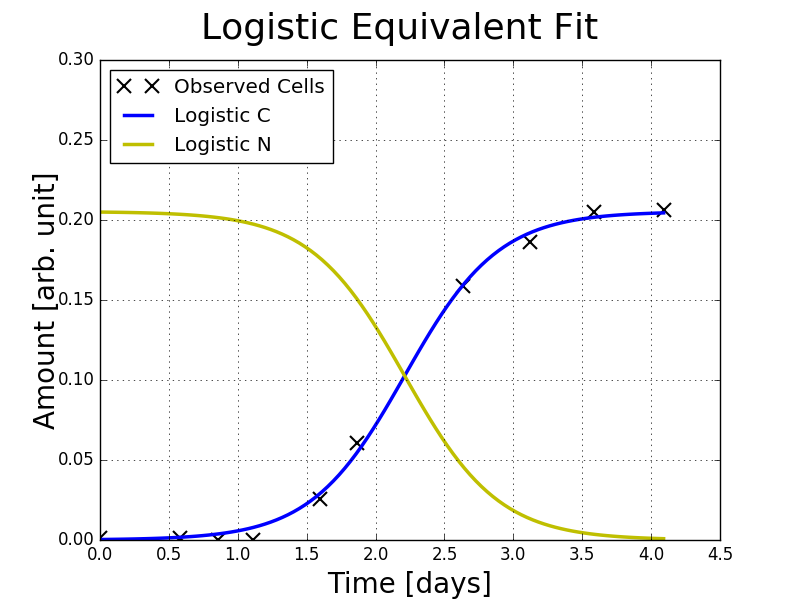
\includegraphics[width=\linewidth]{correction/log_eq_fit}
  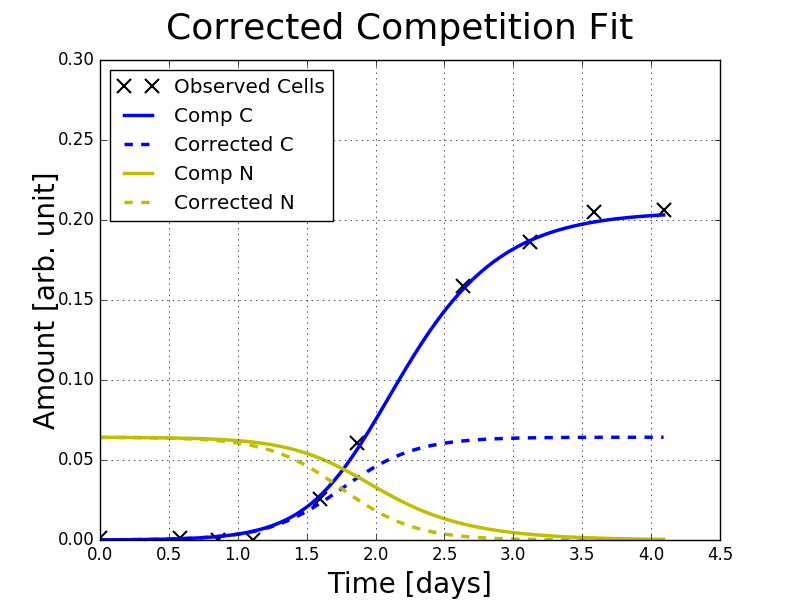
\includegraphics[width=\linewidth]{correction/comp_correction}
  \captionof{figure}{PUT KN VALUES (and r and K) ON THE PLOT. (Could
    even put obj fun values). Fits to culture (R10, C3) of P15
    \citep{Addinall2011} illustrating how the competition model can be
    seen as a correction to the logistic model. \(C\) - Cells; \(N\) -
    Nutrients. Top - Logistic Equivalent Fit; Bottom - Competition Fit
    (solid) and Corrected Logistic Equivalent Fit (dashed).}
  \label{fig:correction}
\end{Figure}

%%% Local Variables:
%%% mode: latex
%%% TeX-master: "report"
%%% End:
